\section{BadUSB-C}

\subsection{Motivation}

\subsection{Implementation}
The implementation of BadUSB-C extends several existing offensive BadUSB device including Rubber Ducky (where we implement the co-operation of HID emulation and screen streaming) and Raspberry Pi (on which we implement the capture of video stream and its processing). We implemented the QR-Code extraction agent from scratch. The complete workflow of BadUSB-C, demonstrating the interaction of all the components is presented at Fig.~\ref{workflow}.

\begin{figure}[htbp]
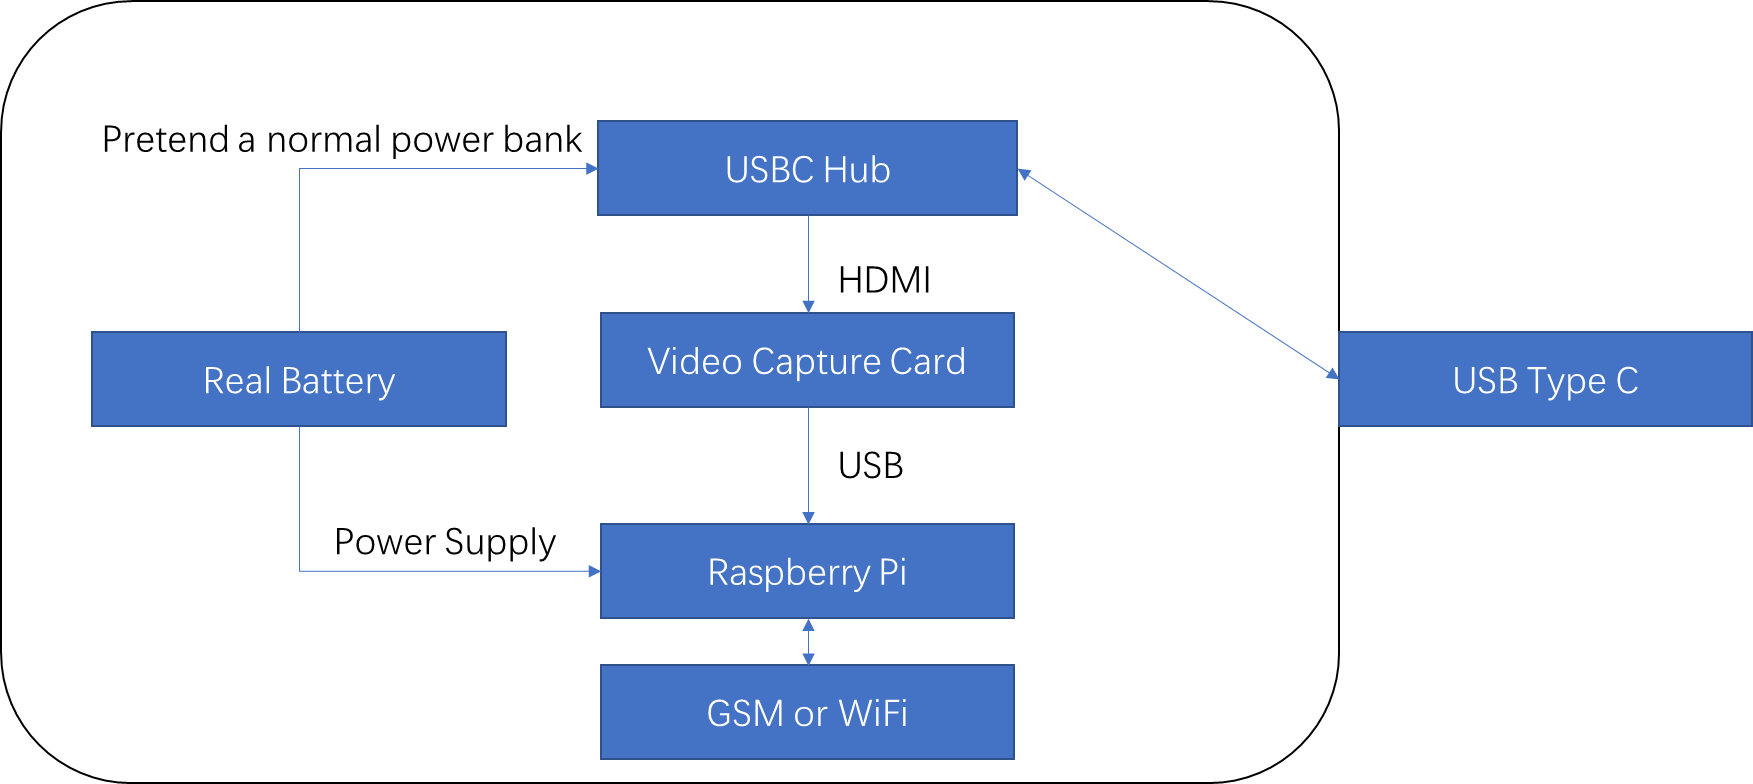
\includegraphics[width=\linewidth]{./Figs/workflow.png}
\caption{Workflow of BadUSB-C}
\label{workflow}
\end{figure}

When the victim plugs in BadUSB-C device, the USB-C hub handles all the communication between each components and the victim's device. Due to the trust-by-default feature of USB protocol, the victim's video stream will be captured. Later, the stream is either processed directly by Raspberry Pi or transmitted to the attacker through GSM/WiFi components.

With video stream the capability of original Rubbery Ducky attack is considerably expanded. For example, the attacker can directly control the victim's device and view the private data in the stream. More details is presented in the Section~\ref{section:experiment}